    \begin{QUESTION}
        \begin{ExamInfo}{93}{學測}{單選}{1}
        \end{ExamInfo}
        \begin{ExamAnsRateInfo}{71}{93}{79}{41}
        \end{ExamAnsRateInfo}
        \begin{QBODY}
            已知一等差數列共有十項,且知其奇數項之和為15,偶數項之和為30,則下列哪一選項為此數列之公差? 
            \begin{QOPS} 
                \QOP 1 
                \QOP 2 
                \QOP 3 
                \QOP 4 
                \QOP 5 
            \end{QOPS}
        \end{QBODY}
        \begin{QFROMS}
        \end{QFROMS}
        \begin{QTAGS}\QTAG{B2C1數列級數}\QTAG{等差級數}\QTAG{B2C1-2級數}\QTAG{B2C1-1數列}\QTAG{等差數列}\end{QTAGS}
        \begin{QANS}
            (3)
        \end{QANS}
        \begin{QSOLLIST}
        \end{QSOLLIST}
        \begin{QEMPTYSPACE}
        \end{QEMPTYSPACE}
    \end{QUESTION}
    \begin{QUESTION}
        \begin{ExamInfo}{93}{學測}{單選}{2}
        \end{ExamInfo}
        \begin{ExamAnsRateInfo}{60}{85}{62}{33}
        \end{ExamAnsRateInfo}
        \begin{QBODY}
            下列選項中的數,何者最大? 
            \begin{QOPS} 
                \QOP $100^{10}$ 
                \QOP $10^{100}$ 
                \QOP $50^{50} $
                \QOP $50!$ 
                \QOP $\frac{100!}{50!}$。 
            \end{QOPS}
        \end{QBODY}
        \begin{QFROMS}
        \end{QFROMS}
        \begin{QTAGS}\QTAG{B1C3-1指數}\QTAG{B1C3指對數函數}\end{QTAGS}
        \begin{QANS}
            (2)
        \end{QANS}
        \begin{QSOLLIST}
        \end{QSOLLIST}
        \begin{QEMPTYSPACE}
        \end{QEMPTYSPACE}
    \end{QUESTION}
    \begin{QUESTION}
        \begin{ExamInfo}{93}{學測}{單選}{3}
        \end{ExamInfo}
        \begin{ExamAnsRateInfo}{44}{76}{40}{16}
        \end{ExamAnsRateInfo}
        \begin{QBODY}
            右圖陰影部分所示為複數平面上區域 $A= \{ z:z=r(\cos \theta +i\sin \theta), 0\leq r \leq 1, \frac{3}{4} \pi \leq \theta \leq \frac{5}{4} \pi \} $ 之略圖。
            令 $D =\{ w:w = z^3 , z \in A\}$,試問下列選項中之略圖,何者之陰影部分與區域 $D$ 最接近?
            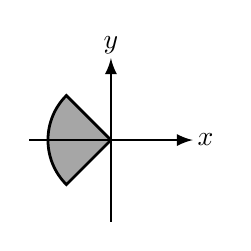
\begin{tikzpicture}[scale=.8]
            \begin{scope}
            \pgfsetlinewidth{1pt}
            \draw[fill=gray!70] (0,0) -- (135:1cm) arc (135:225:1cm) -- (0,0);
            \node at (0,1.5) {$y$};
            \node at (1.5,0) {$x$};
            \pgfsetarrowsend{latex}
            \draw (-1.3,0) to[->] (1.3,0);
            \draw (0,-1.3) to[->] (0,1.3);
            \end{scope}
            \end{tikzpicture}
            \begin{QOPS}
                \QOP 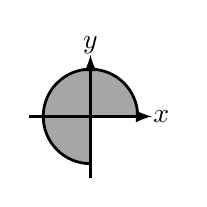
\begin{tikzpicture}[scale=.6]
                    \begin{scope}
                    \pgfsetlinewidth{1pt}
                    \draw[fill=gray!70] (0,0) -- (0:1cm) arc (0:270:1cm) -- (0,0);
                    \node at (0,1.5) {$y$};
                    \node at (1.5,0) {$x$};
                    \pgfsetarrowsend{latex}
                    \draw (-1.3,0) to[->] (1.3,0);
                    \draw (0,-1.3) to[->] (0,1.3);
                    \end{scope}
                    \end{tikzpicture}
                
                \QOP 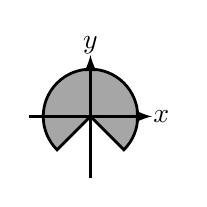
\begin{tikzpicture}[scale=.6]
                    \begin{scope}
                    \pgfsetlinewidth{1pt}
                    \draw[fill=gray!70] (0,0) -- (-45:1cm) arc (-45:225:1cm) -- (0,0);
                    \node at (0,1.5) {$y$};
                    \node at (1.5,0) {$x$};
                    \pgfsetarrowsend{latex}
                    \draw (-1.3,0) to[->] (1.3,0);
                    \draw (0,-1.3) to[->] (0,1.3);
                    \end{scope}
                    \end{tikzpicture}
                    
                \QOP 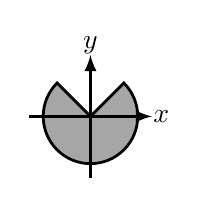
\begin{tikzpicture}[scale=.6]
                    \begin{scope}
                    \pgfsetlinewidth{1pt}
                    \draw[fill=gray!70] (0,0) -- (135:1cm) arc (-225:45:1cm) -- (0,0);
                    \node at (0,1.5) {$y$};
                    \node at (1.5,0) {$x$};
                    \pgfsetarrowsend{latex}
                    \draw (-1.3,0) to[->] (1.3,0);
                    \draw (0,-1.3) to[->] (0,1.3);
                    \end{scope}
                    \end{tikzpicture}
                \QOP 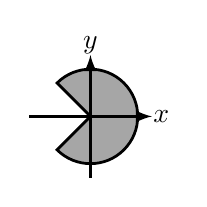
\begin{tikzpicture}[scale=.6]
                \begin{scope}
                \pgfsetlinewidth{1pt}
                \draw[fill=gray!70] (0,0) -- (225:1cm) arc (-135:135:1cm) -- (0,0);
                \node at (0,1.5) {$y$};
                \node at (1.5,0) {$x$};
                \pgfsetarrowsend{latex}
                \draw (-1.3,0) to[->] (1.3,0);
                \draw (0,-1.3) to[->] (0,1.3);
                \end{scope}
                \end{tikzpicture}
                
                \QOP 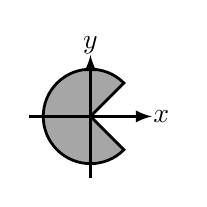
\begin{tikzpicture}[scale=.6]
                    \begin{scope}
                    \pgfsetlinewidth{1pt}
                    \draw[fill=gray!70] (0,0) -- (45:1cm) arc (45:315:1cm) -- (0,0);
                    \node at (0,1.5) {$y$};
                    \node at (1.5,0) {$x$};
                    \pgfsetarrowsend{latex}
                    \draw (-1.3,0) to[->] (1.3,0);
                    \draw (0,-1.3) to[->] (0,1.3);
                    \end{scope}
                    \end{tikzpicture}
            \end{QOPS}
        \end{QBODY}
        \begin{QFROMS}
        \end{QFROMS}
        \begin{QTAGS}\QTAG{B5C2三角函數II}\end{QTAGS}
        \begin{QANS}
            (5)
        \end{QANS}
        \begin{QSOLLIST}
        \end{QSOLLIST}
        \begin{QEMPTYSPACE}
        \end{QEMPTYSPACE}
    \end{QUESTION}
    \begin{QUESTION}
        \begin{ExamInfo}{93}{學測}{單選}{4}
        \end{ExamInfo}
        \begin{ExamAnsRateInfo}{23}{42}{17}{10}
        \end{ExamAnsRateInfo}
        \begin{QBODY}
            在坐標空間中給定兩點 $A(1,2,3)$ 與 $B(7,6,5)$。令 $S$ 為 $xy$- 平面上所有使得向量 $PA$ 垂直於向量 $PB$ 的 $P$ 點所成的集合,則
            \begin{QOPS} 
                \QOP $S$ 為空集合 
                \QOP $S$ 恰含一點 
                \QOP $S$ 恰含兩點 
                \QOP $S$ 為一線段 
                \QOP $S$ 為一圓
            \end{QOPS}
        \end{QBODY}
        \begin{QFROMS}
        \end{QFROMS}
        \begin{QTAGS}\QTAG{B4C1空間向量}\end{QTAGS}
        \begin{QANS}
            (1)
        \end{QANS}
        \begin{QSOLLIST}
        \end{QSOLLIST}
        \begin{QEMPTYSPACE}
        \end{QEMPTYSPACE}
    \end{QUESTION}
    \begin{QUESTION}
        \begin{ExamInfo}{93}{學測}{單選}{5}
        \end{ExamInfo}
        \begin{ExamAnsRateInfo}{61}{88}{62}{33}
        \end{ExamAnsRateInfo}
        \begin{QBODY}
            設 $\triangle ABC$ 為平面上的一個三角形,$P$ 為平面上一點且 $\lvec{AP}= \frac{1}{3}\lvec{AB}+ t\lvec{AC}$,其中 $t$為一實數。
            試問下列哪一選項為 $t$ 的最大範圍,使得 $P$ 落在 $\triangle ABC$ 的內部? 
            \begin{QOPS} 
                \QOP $0<t < \frac{1}{4}$ 
                \QOP $0 < t < \frac{1}{3}$ 
                \QOP $0 < t <\frac{1}{2}$ 
                \QOP $0 < t < \frac{2}{3}$ 
                \QOP $0 < t < \frac{3}{4}$
            \end{QOPS}
        \end{QBODY}
        \begin{QFROMS}
        \end{QFROMS}
        \begin{QTAGS}\QTAG{線性組合}\QTAG{B3C3-1平面向量的表示法}\QTAG{B3C3平面向量}\end{QTAGS}
        \begin{QANS}
            (4)
        \end{QANS}
        \begin{QSOLLIST}
        \end{QSOLLIST}
        \begin{QEMPTYSPACE}
        \end{QEMPTYSPACE}
    \end{QUESTION}
    \begin{QUESTION}
        \begin{ExamInfo}{93}{學測}{單選}{6}
        \end{ExamInfo}
        \begin{ExamAnsRateInfo}{26}{42}{27}{9}
        \end{ExamAnsRateInfo}
        \begin{QBODY}
            台灣證劵交易市場規定股票成交價格只能在前一個交易日的收盤價的漲、跌 $7\%$ 範圍內變動。例如:某支股票前一個交易日的收盤價是每股 100 元,則今天該支股票每股的買賣價格必須在 93 元至 107 元之間。假設有某支股票的價格起伏很大,某一天的收盤價是每股 40 元,次日起連續五個交易日以跌停板收盤 (每天跌 $7\%$),緊接著卻連續五個交易日以漲停板收盤(每天漲 $7\%$)。請問經過這十個交易日後,該支股票每股的收盤價最接近下列哪一個選項中的價格?
            \begin{QOPS}
                \QOP $39$ 元
                \QOP $39.5$ 元
                \QOP $40$ 元
                \QOP $40.5$ 元
                \QOP $41$ 元
            \end{QOPS}
        \end{QBODY}
        \begin{QFROMS}
        \end{QFROMS}
        \begin{QTAGS}\QTAG{應用問題}\QTAG{B1C3指對數函數}\QTAG{B1C3-5指數與對數的應用}\end{QTAGS}
        \begin{QANS}
            (1)
        \end{QANS}
        \begin{QSOLLIST}
        \end{QSOLLIST}
        \begin{QEMPTYSPACE}
        \end{QEMPTYSPACE}
    \end{QUESTION}
    \begin{QUESTION}
        \begin{ExamInfo}{93}{學測}{多選}{7}
        \end{ExamInfo}
        \begin{ExamAnsRateInfo}{56}{77}{61}{30}
        \end{ExamAnsRateInfo}
        \begin{QBODY}
            中山高速公路重慶北路交流道南下入口匝道分成內、外兩線車道,路旁立有標誌 「外側車道 大客車專用」。請選出不違反此規定的選項:
            \begin{QOPS}
                \QOP 小型車行駛內側車道 
                \QOP 小型車行駛外側車道 
                \QOP 大客車行駛內側車道 
                \QOP 大客車行駛外側車道 
                \QOP 大貨車行駛外側車道
            \end{QOPS}
        \end{QBODY}
        \begin{QFROMS}
        \end{QFROMS}
        \begin{QTAGS}\QTAG{邏輯}\QTAG{B2C2-1簡單的邏輯與集合}\QTAG{B2C2排列組合}\end{QTAGS}
        \begin{QANS}
            (1)(3)(4)
        \end{QANS}
        \begin{QSOLLIST}
        \end{QSOLLIST}
        \begin{QEMPTYSPACE}
        \end{QEMPTYSPACE}
    \end{QUESTION}
    \begin{QUESTION}
        \begin{ExamInfo}{93}{學測}{多選}{8}
        \end{ExamInfo}
        \begin{ExamAnsRateInfo}{43}{77}{39}{13}
        \end{ExamAnsRateInfo}
        \begin{QBODY}
            在坐標平面上,下列哪些方程式的圖形可以放進一個夠大的圓裡面? 
            \begin{QOPS} 
                \QOP $3x=2y^2$ 
                \QOP $3x^2+2y^2=1$ 
                \QOP $3x^2-2y^2=1$ \QOP $|x+y|=1$ 
                \QOP $|x|+|y|=1$
            \end{QOPS}
        \end{QBODY}
        \begin{QFROMS}
        \end{QFROMS}
        \begin{QTAGS}\QTAG{跨章節試題}\end{QTAGS}
        \begin{QANS}
            (2)(5)
        \end{QANS}
        \begin{QSOLLIST}
        \end{QSOLLIST}
        \begin{QEMPTYSPACE}
        \end{QEMPTYSPACE}
    \end{QUESTION}
    \begin{QUESTION}
        \begin{ExamInfo}{93}{學測}{多選}{9}
        \end{ExamInfo}
        \begin{ExamAnsRateInfo}{46}{70}{38}{30}
        \end{ExamAnsRateInfo}
        \begin{QBODY}
            如右圖 $O-ABCD$ 為一金字塔,底是邊長為 $1$ 之正方形,
            頂點 $O$ 與 $A$, $B$, $C$, $D$ 之距離均為 2。試問下列哪些式子是正確的?
            \begin{QOPS} 
                \QOP  $\lvec{OA}+\lvec{OB} +\lvec{OC}+\lvec{OD}=\lvec{0}$, 
                \QOP $\lvec{OA} + \lvec{OB}$  $-\lvec{OC}- \lvec{OD} =\lvec{0}$ 
                \QOP $\lvec{OA}- \lvec{OB}+ \lvec{OC} -\lvec{OD}= \lvec{0}$ 
                \QOP $\lvec{OA} \cdot \lvec{OB} = \lvec{OC} \cdot \lvec{OD}$
                \QOP $\lvec{OA}\cdot \lvec{OC}=2$。
            \end{QOPS}
            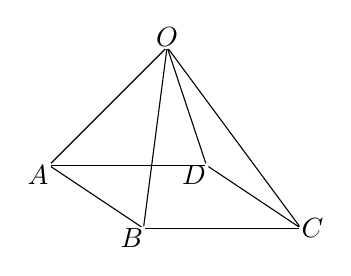
\begin{tikzpicture}[inner sep=0pt]
            \node (v00) at (0,0) {};
            \node[anchor =north east] (t00) at (v00) {$A$};
            \node (v01) at (1.2,-.8) {};
            \node[anchor =north east] (t01) at (v01) {$B$};
            \node (v10) at (2,0) {};
            \node[anchor = north east] (t10) at (v10) {$D$};
            \node (v11) at (3.2,-.8) {};
            \node[anchor =west] (t11) at (v11) {$C$};
            \node (vtop) at (1.5,1.5) {};
            \node[anchor =south] (ttop) at (vtop) {$O$};
            \draw (v00) to (v01);
            \draw (v00) to (v10);
            \draw (v11) to (v01);
            \draw (v11) to (v10);
            \draw (vtop) to (v01);
            \draw (vtop) to (v10);
            \draw (vtop) to (v11);
            \draw (vtop) to (v00);
            \end{tikzpicture}
        \end{QBODY}
        \begin{QFROMS}
        \end{QFROMS}
        \begin{QTAGS}\QTAG{B4C1-2空間向量的坐標表示法}\QTAG{B4C1空間向量}\end{QTAGS}
        \begin{QANS}
            (3)(4)
        \end{QANS}
        \begin{QSOLLIST}
        \end{QSOLLIST}
        \begin{QEMPTYSPACE}
        \end{QEMPTYSPACE}
    \end{QUESTION}
    \begin{QUESTION}
        \begin{ExamInfo}{93}{學測}{多選}{10}
        \end{ExamInfo}
        \begin{ExamAnsRateInfo}{43}{77}{40}{12}
        \end{ExamAnsRateInfo}
        \begin{QBODY}
            從 $1,2,\dots ,10$ 這十個數中隨意取兩個,以 $p$ 表示其和為偶數之機率, $q$ 表示其和為奇數之機率。 試問下列哪些敘述是正確的?
             \begin{QOPS} 
                \QOP $p+q=1$ 
                \QOP $p=q$  
                \QOP $|p-q| \leq \frac{1}{10} $ 
                \QOP $|p-q| \geq \frac{1}{20}$ \QOP $p\geq \frac{1}{2}$
            \end{QOPS}
        \end{QBODY}
        \begin{QFROMS}
        \end{QFROMS}
        \begin{QTAGS}\QTAG{B2C3機率}\QTAG{B2C3-2機率的定義與性質}\end{QTAGS}
        \begin{QANS}
            (1)(4)
        \end{QANS}
        \begin{QSOLLIST}
        \end{QSOLLIST}
        \begin{QEMPTYSPACE}
        \end{QEMPTYSPACE}
    \end{QUESTION}
    \begin{QUESTION}
        \begin{ExamInfo}{93}{學測}{多選}{11}
        \end{ExamInfo}
        \begin{ExamAnsRateInfo}{29}{55}{23}{9}
        \end{ExamAnsRateInfo}
        \begin{QBODY}
            設 $f(x)$ 為三次實係數多項式,且知複數 $1+i$ 為 $f(x)=0$ 之一解,
            試問下列哪些敘述是正確的?
            \begin{QOPS} 
                \QOP $f(1-i)=0$ \quad 
                \QOP $f(2+i) \neq 0$ 
                \QOP 沒有實數解 $x$ 滿足 $f(x)=x$ 
                \QOP 沒有實數解 $x$ 滿足 $f(x^3)=x$ 
                \QOP 若 $f(0)>0$ 且 $f(2) <0$,則 $f(4)<0$ 
            \end{QOPS}
        \end{QBODY}
        \begin{QFROMS}
        \end{QFROMS}
        \begin{QTAGS}\QTAG{B1C2多項式函數}\QTAG{B1C2-3多項式方程式}\QTAG{勘根定理}\QTAG{虛根定理}\QTAG{複數}\end{QTAGS}
        \begin{QANS}
            (1)(2)(5)
        \end{QANS}
        \begin{QSOLLIST}
        \end{QSOLLIST}
        \begin{QEMPTYSPACE}
        \end{QEMPTYSPACE}
    \end{QUESTION}
    \begin{QUESTION}
        \begin{ExamInfo}{93}{學測}{填充}{A}
        \end{ExamInfo}
        \begin{ExamAnsRateInfo}{70}{90}{77}{43}
        \end{ExamAnsRateInfo}
        \begin{QBODY}
            某數學老師計算學期成績的公式如下:五次平時考中取較好的三次之平均值佔 $30\%$,兩次期中考各佔 $20\%$,期末考佔 $30\%$。某生平時考成績分別為 68、82、70、73、85,期中考成績分別為 86、79,期末考成績為 90,則該生學期成績為 
            \TCNBOX{\TCN\TCN}。(計算到整數為止,小數點以後四捨五入)
        \end{QBODY}
        \begin{QFROMS}
        \end{QFROMS}
        \begin{QTAGS}\QTAG{B2C4-1一維數據分析}\QTAG{B2C4數據分析}\QTAG{加權平均數}\end{QTAGS}
        \begin{QANS}
            $84$
        \end{QANS}
        \begin{QSOLLIST}
        \end{QSOLLIST}
        \begin{QEMPTYSPACE}
        \end{QEMPTYSPACE}
    \end{QUESTION}
    \begin{QUESTION}
        \begin{ExamInfo}{93}{學測}{填充}{B}
        \end{ExamInfo}
        \begin{ExamAnsRateInfo}{25}{57}{16}{2}
        \end{ExamAnsRateInfo}
        \begin{QBODY}
            某電視台舉辦抽獎遊戲,現場準備的抽獎箱裡放置了四個分別標有 1000、 800、 600、 0 元獎額的球。
            參加者自行從抽獎箱裡摸取一球(取後即放回),
            主辦單位即贈送與此球上數字等額的獎金,並規定抽取到 0 元的人可以再摸一次,但是所得獎金折半(若再摸到 0 就沒有第三次機會);則一個參加者可得獎金的期望值是 
            \TCNBOX{\TCN\TCN\TCN} 元。(計算到整數為止,小數點以後四捨五入)
        \end{QBODY}
        \begin{QFROMS}
        \end{QFROMS}
        \begin{QTAGS}\QTAG{B5C1機率與統計}\end{QTAGS}
        \begin{QANS}
            $675$
        \end{QANS}
        \begin{QSOLLIST}
        \end{QSOLLIST}
        \begin{QEMPTYSPACE}
        \end{QEMPTYSPACE}
    \end{QUESTION}
    \begin{QUESTION}
        \begin{ExamInfo}{93}{學測}{填充}{C}
        \end{ExamInfo}
        \begin{ExamAnsRateInfo}{36}{77}{27}{4}
        \end{ExamAnsRateInfo}
        \begin{QBODY}
            設 $a,b,c$ 為正整數,若 $a\log_{520} 2+b\log_{520} 5+c\log_{520}13=3$,則 $a+b+c=$ 
            \TCNBOX{} 。
        \end{QBODY}
        \begin{QFROMS}
        \end{QFROMS}
        \begin{QTAGS}\QTAG{B1C3-3對數}\QTAG{B1C3指對數函數}\QTAG{對數律}\end{QTAGS}
        \begin{QANS}
            $15$
        \end{QANS}
        \begin{QSOLLIST}
        \end{QSOLLIST}
        \begin{QEMPTYSPACE}
        \end{QEMPTYSPACE}
    \end{QUESTION}
    \begin{QUESTION}
        \begin{ExamInfo}{93}{學測}{填充}{D}
        \end{ExamInfo}
        \begin{ExamAnsRateInfo}{19}{45}{8}{4}
        \end{ExamAnsRateInfo}
        \begin{QBODY}
            設 $\triangle ABC$ 為一等腰直角三角形,$\angle BAC = 90^\circ$ 。
            若 $P$, $Q$ 為斜邊 $\overline{BC}$ 的三等分點,則 $\tan \angle PAQ = $
            \TCNBOX{\TCN\TCN} 。
        \end{QBODY}
        \begin{QFROMS}
        \end{QFROMS}
        \begin{QTAGS}\QTAG{B3C3-2平面向量的內積}\QTAG{B3C3平面向量}\QTAG{夾角}\end{QTAGS}
        \begin{QANS}
            $\frac{3}{4}$
        \end{QANS}
        \begin{QSOLLIST}
        \end{QSOLLIST}
        \begin{QEMPTYSPACE}
        \end{QEMPTYSPACE}
    \end{QUESTION}
    \begin{QUESTION}
        \begin{ExamInfo}{93}{學測}{填充}{E}
        \end{ExamInfo}
        \begin{ExamAnsRateInfo}{52}{77}{56}{23}
        \end{ExamAnsRateInfo}
        \begin{QBODY}
            某高中招收高一新生共有男生 1008 人、女生 924 人報到。學校想將他們依男女合班的原則平均分班,且要求各班有同樣多的男生,也有同樣多的女生;考量教學效益,並限制各班總人數在 40 與 50 人之間,則共分成	
            \TCNBOX{\TCN\TCN} 班。
        \end{QBODY}
        \begin{QFROMS}
        \end{QFROMS}
        \begin{QTAGS}\QTAG{不是99課綱}\end{QTAGS}
        \begin{QANS}
            $42$
        \end{QANS}
        \begin{QSOLLIST}
        \end{QSOLLIST}
        \begin{QEMPTYSPACE}
        \end{QEMPTYSPACE}
    \end{QUESTION}
    \begin{QUESTION}
        \begin{ExamInfo}{93}{學測}{填充}{F}
        \end{ExamInfo}
        \begin{ExamAnsRateInfo}{26}{61}{15}{2}
        \end{ExamAnsRateInfo}
        \begin{QBODY}
            在坐標空間中,平面 $x-2y+z=0$ 上有一以點 $P(1,1,1)$ 為圓心的圓 $\Gamma$ ,
            而 $Q(-9,9, 27)$ 為圓 $\Gamma$ 上 一點。
            若過 $Q$ 與圓  $\Gamma$ 相切的直線之一方向向量為 $(a, b, 1)$,則 $a= 
            \TCNBOX{\TCN}$, $b= 
            \TCNBOX{\TCN}$。
        \end{QBODY}
        \begin{QFROMS}
        \end{QFROMS}
        \begin{QTAGS}\QTAG{B4C2空間中的平面與直線}\QTAG{B4C2-1平面方程式}\end{QTAGS}
        \begin{QANS}
            $a=5, b=3$
        \end{QANS}
        \begin{QSOLLIST}
        \end{QSOLLIST}
        \begin{QEMPTYSPACE}
        \end{QEMPTYSPACE}
    \end{QUESTION}
    \begin{QUESTION}
        \begin{ExamInfo}{93}{學測}{填充}{G}
        \end{ExamInfo}
        \begin{ExamAnsRateInfo}{10}{27}{3}{0}
        \end{ExamAnsRateInfo}
        \begin{QBODY}
            設 $270^\circ <A< 360^\circ$ 且 $\sqrt{3}\sin A+ \cos A=2 \sin {2004} ^\circ$。若 $A=m^\circ$,則 $m=$
            \TCNBOX{\TCN\TCN\TCN}。
        \end{QBODY}
        \begin{QFROMS}
        \end{QFROMS}
        \begin{QTAGS}\QTAG{B5C2三角函數II}\QTAG{B5C2-2三角函數的應用}\end{QTAGS}
        \begin{QANS}
            $306$
        \end{QANS}
        \begin{QSOLLIST}
        \end{QSOLLIST}
        \begin{QEMPTYSPACE}
        \end{QEMPTYSPACE}
    \end{QUESTION}
    \begin{QUESTION}
        \begin{ExamInfo}{93}{學測}{填充}{H}
        \end{ExamInfo}
        \begin{ExamAnsRateInfo}{21}{37}{18}{8}
        \end{ExamAnsRateInfo}
        \begin{QBODY}
            坐標平面上的圓 $C:(x-7)^2+(y-8)^2=9$ 上有 
            \TCNBOX{\TCN\TCN} 個點與原點的距離正好是整數值。
        \end{QBODY}
        \begin{QFROMS}
        \end{QFROMS}
        \begin{QTAGS}\QTAG{B3C2-3圓與直線的關係}\QTAG{圖形}\QTAG{B3C2直線與圓}\end{QTAGS}
        \begin{QANS}
            $12$
        \end{QANS}
        \begin{QSOLLIST}
        \end{QSOLLIST}
        \begin{QEMPTYSPACE}
        \end{QEMPTYSPACE}
    \end{QUESTION}
    \begin{QUESTION}
        \begin{ExamInfo}{93}{學測}{填充}{I}
        \end{ExamInfo}
        \begin{ExamAnsRateInfo}{19}{47}{7}{3}
        \end{ExamAnsRateInfo}
        \begin{QBODY}
            在坐標平面上,設直線 $L:y=x+2$ 與拋物線 $\Gamma :x^2=4y$ 相交於 $P,Q$ 兩點。若 $F$ 表拋物線 $\Gamma$ 的焦點,則 $\overline{PF}+\overline{QF}=$ 
            $\TCNBOX{\TCN\TCN}$
        \end{QBODY}
        \begin{QFROMS}
        \end{QFROMS}
        \begin{QTAGS}\QTAG{B4C4二次曲線}\QTAG{B4C4-1拋物線}\QTAG{圖形}\end{QTAGS}
        \begin{QANS}
            $10$
        \end{QANS}
        \begin{QSOLLIST}
        \end{QSOLLIST}
        \begin{QEMPTYSPACE}
        \end{QEMPTYSPACE}
    \end{QUESTION}
